\subsection{OpenMP: memoria condivisa}
\label{sec:openmp}

Nel modello a memoria condivisa i thread non si scambiano dati in modo
esplicito: leggono e scrivono la stessa matrice degli escape time,
residente in un unico spazio di indirizzamento. Il grado di parallelismo non è
quindi fissato dal numero di pixel --- che sono milioni --- ma dal numero di
core del nodo: OpenMP istanzia un pool fisso di thread, e le clausole di
schedule non regolano \emph{quanti} thread esistano, bensì la granularità con
cui il lavoro viene ripartito tra essi.

Sebbene nella sezione~\ref{sec:parallelizzazione} si sia individuato nel
singolo pixel l'unità indipendente della computazione, non conviene farne
l'unità di \emph{ripartizione}. Assegnare un pixel per volta a ciascun thread
introduce due costi che si sommano senza aggiungere parallelismo. Primo, un
costo di scheduling: ogni prelievo di una nuova unità richiede un accesso a un
contatore condiviso, e per un'unità da poche centinaia di iterazioni tale costo
non è trascurabile rispetto al calcolo stesso. Secondo, il \emph{false sharing}: pixel
adiacenti sulla stessa riga cadono nella medesima cache line, che rimbalzerebbe
tra i core scriventi.

Si ripartisce quindi il ciclo esterno, sulle righe: a ciascun thread è
assegnato un gruppo di righe intere. Il costo di scheduling viene così
ammortizzato sui pixel della riga, e il false sharing si riduce alle sole righe
di confine fra due gruppi, dove l'ultimo pixel di una riga e il primo della
successiva possono condividere una cache line: un effetto trascurabile.

La decomposizione per righe rende anche immediata la correttezza. Ogni thread
scrive esclusivamente nelle celle delle proprie righe: gli insiemi di celle
scritte sono disgiunti, non esiste alcuna \emph{race condition} sui dati e non
è necessaria alcuna sincronizzazione in scrittura. Il false sharing residuo è
un problema di prestazioni, non di correttezza. La coincidenza del
checksum con quello della baseline seriale è la verifica sperimentale di questa
assenza di race: una sovrapposizione in scrittura altererebbe la matrice e il
checksum non tornerebbe.

% ============================================================
\subsubsection{Design dello sweep}
\label{sec:openmp-sweep}
% ============================================================

La domanda progettuale non è quanto parallelizzare, ma \emph{con quale regola
assegnare le righe ai thread}. La risposta non è unica: esistono politiche con
proprietà di bilanciamento e di coordinamento molto diverse, e confrontarle
empiricamente è l'obiettivo dell'esperimento. Lo sweep sistema cinque politiche
sullo stesso intervallo di $p \in \{2, 4, 8, 16, 32\}$ thread, a griglia
$1024^2$ e $N_{\max} = 1000$ fissati: variare le sole leve di scheduling
isola l'effetto della politica da quello del carico e del numero di core.

\paragraph{\texttt{static}.}
Assegna in anticipo a ogni thread un blocco contiguo di $H/p$
righe consecutive. La distribuzione è decisa prima di iniziare: non esiste coda
a runtime, il costo di coordinamento è zero. Il prezzo è che un thread che
esaurisce il proprio blocco resta inattivo fino a che l'ultimo thread non ha
terminato il suo. Poiché le righe che attraversano l'interno dell'insieme
costano fino a $N_{\max}$ iterazioni per pixel mentre quelle ai bordi sfuggono
in poche iterazioni, i blocchi centrali concentrano il lavoro. \texttt{static}
è quindi il caso limite in cui il bilanciamento è interamente delegato alla
geometria del problema: con un profilo di carico uniforme sarebbe ottimale; con
il profilo del Mandelbrot è fortemente sfavorevole. È precisamente questo confronto che motiva la
scelta della politica come primo estremo dello sweep.

\paragraph{\texttt{dynamic} con chunk variabile.}
Invece di assegnare tutto il lavoro in anticipo, il runtime mantiene una coda
di chunk: quando un thread ha esaurito le righe che stava elaborando, preleva il
chunk successivo. Il ribilanciamento è automatico: i thread veloci --- quelli
che hanno elaborato righe leggere --- riprendono subito lavoro, mentre quelli
lenti restano occupati senza lasciare altri in attesa.

La dimensione del chunk governa un compromesso tra due costi opposti. Un chunk
piccolo garantisce un bilanciamento quasi perfetto --- nessun thread può restare
bloccato su un blocco pesante a lungo --- ma moltiplica il numero di accessi
alla coda condivisa, ciascuno dei quali richiede un'operazione di
sincronizzazione interna. Un chunk grande riduce l'overhead di coordinamento,
ma riavvicina il comportamento a quello statico: un thread potrebbe caricarsi di
$k$ righe tutte pesanti e diventare il collo di bottiglia. Per rendere visibile
questo trade-off lo sweep campiona tre valori: $k \in \{1, 16, 64\}$ righe.
\texttt{dynamic,1} è l'estremo di bilanciamento massimo, \texttt{dynamic,64}
quello di overhead minimo; \texttt{dynamic,16} è il punto intermedio. Il chunk
ottimale --- quello che minimizza il tempo complessivo --- emerge dai dati e
costituisce un risultato dell'analisi, non un'ipotesi.

\paragraph{\texttt{guided}.}
È il compromesso adattivo tra i due estremi. Come \texttt{dynamic}, mantiene
una coda; a differenza di esso, la dimensione del chunk non è fissa: parte
proporzionale al lavoro rimasto e si riduce nel tempo. All'inizio, quando ci
sono molte righe disponibili, il chunk è ampio --- l'overhead di coda è basso
come in \texttt{static}. Verso la fine, quando rimangono poche righe e il
rischio è che un thread si trovi con un blocco pesante mentre gli altri sono
fermi, il chunk si rimpicciolisce, replicando la granularità fine di
\texttt{dynamic,1} nel momento in cui conta di più. L'idea è ottenere il
bilanciamento di \texttt{dynamic} pagando una frazione dell'overhead.

% ============================================================
\subsubsection{Metriche specifiche}
\label{sec:openmp-metriche}
% ============================================================

OpenMP non introduce metriche proprie: speedup, efficienza e $e(p)$ restano
quelle comuni della sezione~\ref{sec:metriche-comuni}, calcolate sui soli tempi.
Ciò che è specifico del paradigma è il legame fra la politica di scheduling e lo
sbilanciamento previsto dal profilo seriale. In questo quadro $\mathrm{CoV}$ è
l'indicatore che stabilisce \emph{a priori} se lo scheduling dinamico convenga:
un valore elevato segnala una dispersione del carico tale da giustificarne il
costo di coordinamento, mentre un valore prossimo a zero renderebbe già ottimale
la politica statica.

% ============================================================
\subsubsection{Frammenti di codice rilevanti}
\label{sec:openmp-codice}
% ============================================================

Rispetto al kernel seriale il file OpenMP differisce per due sole righe di
codice, la direttiva sul ciclo esterno e l'etichetta che identifica il paradigma
nel CSV; le funzioni di supporto restano identiche byte per byte, ed è questo a
garantire
la coincidenza del checksum. Qui si commentano solo le scelte rilevanti; il
codice completo è in \repofile{mandelbrot/src/mandelbrot_omp.cpp}.

La differenza sostanziale è una singola direttiva sul ciclo esterno:

\begin{verbatim}
#pragma omp parallel for schedule(runtime)
for (int row = 0; row < computed_rows; ++row) {
    // inner column loop: identical to the serial kernel
    ...
}
\end{verbatim}

Non è necessaria alcuna clausola di data-sharing: le variabili dichiarate nel
corpo del ciclo sono private per costruzione, mentre la matrice è condivisa ma
scritta da ogni thread solo sulle celle delle proprie righe. La scelta
implementativa che conta è \texttt{schedule(runtime)}: la politica non è
fissata nel codice ma letta a esecuzione dalla variabile d'ambiente
\texttt{OMP\_SCHEDULE}, così che un unico binario copra tutte le politiche
variando solo il job script, senza ricompilazione. Il confronto tra politiche è
dunque uno sweep di configurazioni sullo stesso eseguibile, non binari distinti.

Lo sweep è eseguito da un unico job SLURM su un singolo nodo e si ferma a $32$
thread, la capienza di un socket (sezione~\ref{sec:ambiente}). I thread sono
ancorati ai core (\texttt{OMP\_PLACES=cores}, \texttt{OMP\_PROC\_BIND=close}),
così che l'intera campagna resti in un solo dominio NUMA e che la migrazione dei
thread non aggiunga rumore al tempo minimo. Il tempo $T_1$ è misurato nello
stesso job con il binario seriale, e non con la versione OpenMP a un thread, e
tutte le misure usano il kernel \emph{bare}.

% ============================================================
\subsubsection{Analisi dei risultati}
\label{sec:openmp-risultati}
% ============================================================

Il confronto mette a sistema le cinque politiche sullo stesso intervallo di $p$
(da $2$ a $32$ thread), a risoluzione e $N_{\max}$ fissati. La
tabella~\ref{tab:openmp-schedule} raccoglie i $25$ punti misurati, e la
figura~\ref{fig:openmp-schedules} ne riporta gli speedup.
\vspace{2,5mm}
\begin{table}[htbp]
    \centering
    \begin{tabular}{lrrrrr}
        \hline
        Politica & $p$ & $T_\parallel(p)$ [s] & $S(p)$ & $E(p)$ & $e(p)$ \\
        \hline
        seriale & 1 & $0{,}72563$ & --- & --- & --- \\
        \hline
        \texttt{static} & 2  & $0{,}36076$ & $2{,}011$  & $1{,}006$ & $-0{,}0056$ \\
        \texttt{static} & 4  & $0{,}34035$ & $2{,}132$  & $0{,}533$ & $0{,}2921$ \\
        \texttt{static} & 8  & $0{,}21280$ & $3{,}410$  & $0{,}426$ & $0{,}1923$ \\
        \texttt{static} & 16 & $0{,}11748$ & $6{,}176$  & $0{,}386$ & $0{,}1060$ \\
        \texttt{static} & 32 & $0{,}06048$ & $11{,}999$ & $0{,}375$ & $0{,}0538$ \\
        \hline
        \texttt{dynamic,1} & 2  & $0{,}36079$ & $2{,}011$  & $1{,}006$ & $-0{,}0056$ \\
        \texttt{dynamic,1} & 4  & $0{,}18043$ & $4{,}022$  & $1{,}005$ & $-0{,}0018$ \\
        \texttt{dynamic,1} & 8  & $0{,}09028$ & $8{,}037$  & $1{,}005$ & $-0{,}0007$ \\
        \texttt{dynamic,1} & 16 & $0{,}04542$ & $15{,}977$ & $0{,}999$ & $0{,}0001$ \\
        \texttt{dynamic,1} & 32 & $0{,}02342$ & $30{,}988$ & $0{,}968$ & $0{,}0011$ \\
        \hline
        \texttt{dynamic,16} & 2  & $0{,}36091$ & $2{,}011$  & $1{,}005$ & $-0{,}0053$ \\
        \texttt{dynamic,16} & 4  & $0{,}18041$ & $4{,}022$  & $1{,}006$ & $-0{,}0018$ \\
        \texttt{dynamic,16} & 8  & $0{,}09132$ & $7{,}946$  & $0{,}993$ & $0{,}0010$ \\
        \texttt{dynamic,16} & 16 & $0{,}04821$ & $15{,}050$ & $0{,}941$ & $0{,}0042$ \\
        \texttt{dynamic,16} & 32 & $0{,}03126$ & $23{,}211$ & $0{,}725$ & $0{,}0122$ \\
        \hline
        \texttt{dynamic,64} & 2  & $0{,}36073$ & $2{,}012$  & $1{,}006$ & $-0{,}0057$ \\
        \texttt{dynamic,64} & 4  & $0{,}18678$ & $3{,}885$  & $0{,}971$ & $0{,}0099$ \\
        \texttt{dynamic,64} & 8  & $0{,}11765$ & $6{,}168$  & $0{,}771$ & $0{,}0424$ \\
        \texttt{dynamic,64} & 16 & $0{,}11746$ & $6{,}178$  & $0{,}386$ & $0{,}1060$ \\
        \texttt{dynamic,64} & 32 & $0{,}11767$ & $6{,}167$  & $0{,}193$ & $0{,}1351$ \\
        \hline
        \texttt{guided} & 2  & $0{,}36056$ & $2{,}012$  & $1{,}006$ & $-0{,}0062$ \\
        \texttt{guided} & 4  & $0{,}26171$ & $2{,}773$  & $0{,}693$ & $0{,}1475$ \\
        \texttt{guided} & 8  & $0{,}13250$ & $5{,}477$  & $0{,}685$ & $0{,}0658$ \\
        \texttt{guided} & 16 & $0{,}06511$ & $11{,}144$ & $0{,}697$ & $0{,}0290$ \\
        \texttt{guided} & 32 & $0{,}03315$ & $21{,}892$ & $0{,}684$ & $0{,}0149$ \\
        \hline
    \end{tabular}
    \caption{OpenMP: tempo, speedup, efficienza e frazione seriale sperimentale per
    ogni combinazione (politica, chunk, thread). Griglia $1024^2$, $N_{\max}=1000$,
        kernel \emph{bare}, un socket di un unico nodo, minimo su $R=5$ ripetizioni.
        Tutte le righe condividono lo stesso checksum della baseline seriale.}
    \label{tab:openmp-schedule}
\end{table}
\begin{figure}[htbp]
    \centering
    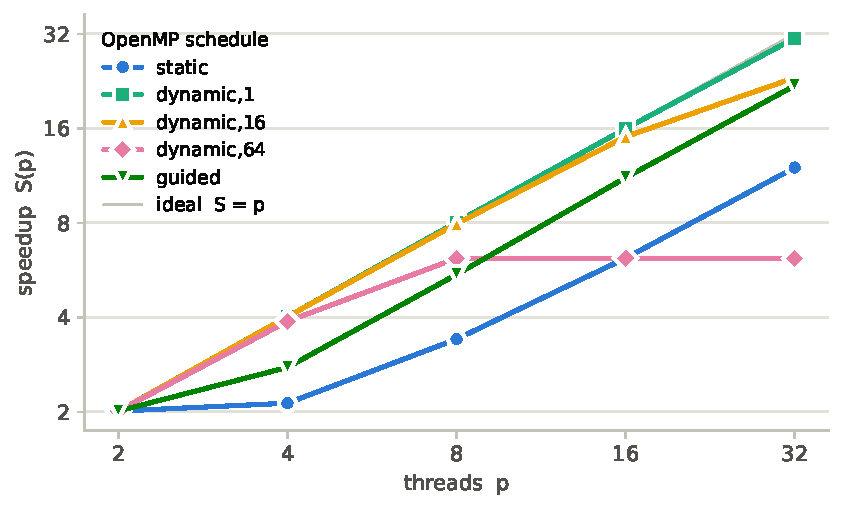
\includegraphics[width=0.85\textwidth]{Immagini/grafici/openmp_schedules}
    \caption{Speedup delle cinque politiche OpenMP in funzione del numero di
    thread, su assi logaritmici in base $2$, con la retta ideale $S = p$. I dati
    sono quelli della tabella~\ref{tab:openmp-schedule}.}
    \label{fig:openmp-schedules}
\end{figure}
\vspace{2,5mm}
Il dato d'insieme è la dispersione: a $32$ thread, sullo stesso hardware e sullo
stesso identico carico, la politica migliore è cinque volte più veloce della
peggiore. L'ordinamento a $p = 32$ è \texttt{dynamic,1} ($S = 30{,}99$),
\texttt{dynamic,16} ($23{,}21$), \texttt{guided} ($21{,}89$), \texttt{static}
($12{,}00$), \texttt{dynamic,64} ($6{,}17$). Poiché il lavoro da svolgere è
identico in tutti i casi --- stessa matrice, stesso checksum ---, il divario
dipende soltanto da come il lavoro è distribuito fra i thread: dall'inattività di
chi resta senza righe e, in misura minore, dal costo di coordinamento. A parità di
kernel, la scelta della politica vale dunque un fattore cinque.

\paragraph{La granularità può annullare il bilanciamento dinamico.}
Il caso più istruttivo della tabella è \texttt{dynamic,64}, che a $8$, $16$ e
$32$ thread restituisce lo stesso tempo a tre cifre significative
($0{,}11765$, $0{,}11746$, $0{,}11767$~s): raddoppiare e poi riquadruplicare i
thread non produce alcun guadagno. La spiegazione è quantitativa e si legge
nella tabella di previsione~\ref{tab:serial_pred_lambdaP}. Con chunk da $64$
righe su $1024$ esistono soltanto $16$ chunk, ciascuno dei quali è un blocco
contiguo; il makespan non può scendere sotto il chunk più pesante, e il peso del
più pesante fra $16$ blocchi contigui è precisamente ciò che misura $\lambda_p$
a $p=16$, da cui il tetto $6{,}169$. Il valore misurato è $6{,}167$. La soglia
cade dove la quota equa $\mathcal{W}/p$ scende sotto il chunk massimo, cioè
attorno a $p=7$: da lì in avanti aggiungere thread non cambia nulla, e a $32$
thread se ne stanno usando in pratica sei.

Se ne ricava una regola generale utile anche altrove: \emph{per uno scheduling
dinamico a chunk fissi di $c$ righe, il tetto allo speedup è quello della
decomposizione a blocchi con $H/c$ blocchi}, indipendentemente dal numero di
thread. Uno scheduling dinamico con grana troppo grossa degenera in uno
scheduling statico con pochi blocchi, e ne eredita per intero lo sbilanciamento
pagando in più il costo della coda.

\paragraph{Il chunk unitario e il costo del coordinamento.}
All'estremo opposto, \texttt{dynamic,1} raggiunge $30{,}99$ su $32$ thread, cioè
il $96{,}8\%$ dell'ideale, con $88{,}7$~GFLOP/s contro i $2{,}86$ del seriale.
Le $1024$ righe formano una coda abbastanza fine da assorbire completamente
l'irregolarità: la sua $e(p)$ resta sotto $0{,}0011$ ovunque, da uno a due
ordini di grandezza più piccola di quella dello statico. Il costo di coordinamento non è
però nullo, e diventa visibile proprio dove il bilanciamento è perfetto: fra
$p=16$ e $p=32$ l'efficienza scende da $0{,}999$ a $0{,}968$, ed è l'unico
punto della campagna in cui \texttt{dynamic,1} si scosta apprezzabilmente
dall'ideale. Con $1024$ prelievi da un contatore condiviso fra $32$ thread, la
contesa sulla coda comincia a farsi sentire. Il confronto con
\texttt{dynamic,16}, che a $32$ thread si ferma a $23{,}21$, mostra che il chunk
deve essere abbastanza piccolo da bilanciare: qui il guadagno di bilanciamento fra
$16$ righe e una riga supera il costo aggiuntivo della coda, perché il carico è
molto irregolare ($\mathrm{CoV} \approx 0{,}97$). Su un carico uniforme ci si
attenderebbe l'esito opposto, ed è questo il senso di $\mathrm{CoV}$ come
indicatore a priori.

\paragraph{\texttt{guided} perde per costruzione, non per overhead.}
La politica \texttt{guided} mostra un'efficienza notevolmente stabile
($0{,}693$, $0{,}685$, $0{,}697$, $0{,}684$ da $4$ a $32$ thread): perde circa
il $31\%$ e lo perde allo stesso modo a ogni grado di parallelismo. Un difetto
di overhead crescerebbe con $p$; una frazione seriale darebbe una $e(p)$
costante, mentre qui $e(p)$ decresce ($0{,}1475 \to 0{,}0149$). Il difetto è
strutturale: \texttt{guided} inizia assegnando chunk proporzionali
alle righe rimanenti, cioè blocchi contigui grandi, e i blocchi contigui in
questo problema ereditano la montagna centrale. I chunk fini, che sarebbero
quelli capaci di bilanciare, arrivano solo alla fine, quando non resta lavoro
con cui compensare. Il caso $p=4$ è il più netto: $2{,}773$ contro i $4{,}022$
di \texttt{dynamic,16}, un divario del $31\%$ fra due politiche entrambe
dinamiche. \texttt{guided} è progettata per ridurre l'overhead di coda su
carichi \emph{quasi} bilanciati; qui il carico è tutt'altro, e la sua euristica
lavora contro il problema.

\paragraph{Throughput assoluto.}
Le metriche viste finora sono tutte \emph{relative}: $S$, $E$ ed $e$ sono
rapporti a $T_1$, e per costruzione non dicono nulla su quanto valga $T_1$
stesso. Il throughput $\Pi(p)$ definito nella sezione~\ref{sec:lavoro}
è l'unica colonna assoluta della campagna, perché il numeratore
$F = \varphi\,\mathcal{W} = 2{,}077\cdot10^{9}$ FLOP è la medesima quantità
analitica per ogni variante --- discende dalla matrice degli escape time, non
dall'implementazione. A $32$ thread le cinque politiche danno

\begin{center}
\begin{tabular}{lrrrrr}
    \hline
    & \texttt{dynamic,1} & \texttt{dynamic,16} & \texttt{guided} & \texttt{static} & \texttt{dynamic,64} \\
    \hline
    $\Pi(32)$ [GFLOP/s] & $88{,}71$ & $66{,}45$ & $62{,}67$ & $34{,}35$ & $17{,}65$ \\
    \hline
\end{tabular}
\end{center}

\noindent contro i $2{,}86$~GFLOP/s del kernel seriale. Come metrica di scaling
$\Pi$ non aggiunge nulla --- il rapporto $\Pi(p)/\Pi(1)$ \emph{è} lo speedup,
per definizione --- ma rende visibile in valore assoluto ciò che la colonna $S$
esprime in rapporto, e soprattutto è la valuta comune con cui la
sezione~\ref{sec:cuda} confronterà CPU e GPU, dove il rapporto con il picco
teorico dell'hardware diventa la domanda centrale. Qui quel confronto non è
proponibile, perché il picco del nodo di calcolo non è stato caratterizzato, e
non lo si stima: $\Pi$ resta un termine di paragone \emph{fra le misure}, non
con il silicio.

Il caso che il throughput illustra meglio è \texttt{dynamic,64}, la cui curva
$\Pi$ si inchioda a $17{,}66$, $17{,}68$, $17{,}65$~GFLOP/s a $8$, $16$ e $32$
thread: il tetto di granularità discusso sopra, espresso in valore assoluto.

\paragraph{Lo statico satura il limite predetto.}
I dati di \texttt{static} si confrontano con il limite $p/\lambda_p$ calcolato
dal profilo seriale; la verifica quantitativa è riportata nella
sezione~\ref{sec:validazione-previsioni}, dove lo stesso confronto è esteso alle
decomposizioni MPI. Anticipando il risultato: l'accordo è entro lo $0{,}6\%$ su
tutti e cinque i punti, confermando che la perdita di efficienza è interamente
attribuibile allo sbilanciamento strutturale e non a overhead di OpenMP.

\paragraph{Lettura di Karp--Flatt.}
Delle tre firme classificate nella sezione~\ref{sec:metriche-comuni} le cinque
politiche ne esibiscono due soltanto, e l'assente è già un risultato: nessuna
mostra $e(p)$ \emph{costante}, cioè in nessun caso la perdita è imputabile a una
frazione seriale genuina --- coerentemente con un kernel che non ne contiene
alcuna. Tutto ciò che $e(p)$ registra qui è sbilanciamento oppure coordinamento,
e la direzione della metrica basta a separarli, purché la si legga insieme alla
forma del tetto e non da sola.
\vspace{2,5mm}
\begin{table}[htbp]
    \centering
    \begin{tabular}{llll}
        \hline
        Politica & $E(p)$, $p \ge 4$ & $e(p)$ & Meccanismo \\
        \hline
        \texttt{static}     & $0{,}533 \to 0{,}375$      & decresce, $0{,}2921 \to 0{,}0538$  & sbilanciamento strutturale \\
        \texttt{guided}     & $\approx 0{,}690$ costante & decresce, $0{,}1475 \to 0{,}0149$  & sbilanciamento strutturale \\
        \texttt{dynamic,1}  & $1{,}005 \to 0{,}968$      & cresce, $-0{,}0018 \to 0{,}0011$   & contesa sulla coda \\
        \texttt{dynamic,16} & $1{,}006 \to 0{,}725$      & cresce, $-0{,}0018 \to 0{,}0122$   & tetto di granularità \\
        \texttt{dynamic,64} & $0{,}971 \to 0{,}193$      & cresce, $0{,}0099 \to 0{,}1351$    & tetto di granularità \\
        \hline
    \end{tabular}
    \caption{OpenMP: classificazione delle cinque politiche secondo l'andamento
    di $e(p)$. L'efficienza è riportata sull'intervallo $p \ge 4$, che esclude
    il punto $p = 2$ affetto dallo scarto di $T_1$ discusso più avanti. Nessuna riga esibisce $e(p)$ costante: la frazione seriale
    nominale del kernel è nulla.}
    \label{tab:openmp-karp-flatt}
\end{table}

\medskip
\noindent\emph{Le politiche a $e(p)$ decrescente.}
\texttt{static} e \texttt{guided} condividono la stessa firma: un'efficienza che
si stabilizza su un valore $E_\infty < 1$ e una $e(p)$ che, sostituendo
$S = p\,E_\infty$ in~\eqref{eq:karp-flatt}, vale
\[
    e(p) = \frac{1/E_\infty - 1}{p - 1} \xrightarrow[p \to \infty]{} 0 .
\]
\texttt{guided} ne è l'esempio più puro, perché la sua efficienza è costante già
a $p = 4$ ($0{,}693$, $0{,}685$, $0{,}697$, $0{,}684$): con
$E_\infty = 0{,}690$ la formula predice $0{,}1500$, $0{,}0643$, $0{,}0300$,
$0{,}0145$ contro i misurati $0{,}1475$, $0{,}0658$, $0{,}0290$, $0{,}0149$. È
la conferma quantitativa di quanto osservato sopra: \texttt{guided} perde il
$31\%$ e lo perde allo stesso modo a ogni grado di parallelismo, il che è
incompatibile con un difetto di overhead.

Per \texttt{static} l'efficienza sta ancora scendendo verso il proprio asintoto
$1/\lambda = 0{,}362$, e conviene perciò usare la forma esatta. La politica
satura il proprio limite (sezione~\ref{sec:validazione-previsioni}), cioè
$S(p) = p/\lambda_p$, da cui
\[
    e(p) = \frac{\lambda_p - 1}{p - 1}
    \qquad
    (0{,}2933,\ 0{,}1927,\ 0{,}1062,\ 0{,}0536 \text{ per } p = 4, 8, 16, 32),
\]
che riproduce i valori misurati entro lo $0{,}5\%$. Poiché $\lambda_p$ è limitato
superiormente dal valore intrinseco $\lambda = 2{,}76$, anche qui la metrica
tende a \emph{zero}. Non c'è dunque alcun tetto fisso che lo statico stia
saturando: il valore $12{,}02$ è il limite \emph{alla singola taglia} $p = 32$,
non un asintoto, perché il tetto della decomposizione a blocchi vale
$p/\lambda_p$ e cresce con $p$, fino a $H/\lambda \approx 370$ nel caso limite
$p = H$. A distinguere i due casi è la \emph{direzione} della metrica, non il suo
valore: un tetto fisso $S_{\max}$ dà una $e(p)$ \emph{crescente}, che converge a
$1/S_{\max}$ dal basso --- è quanto si osserva più avanti per \texttt{dynamic,64}
--- mentre qui $e(p)$ decresce di un fattore cinque. Il confronto fra
$e(32) = 0{,}0538$ e $1/12{,}02 \approx 0{,}083$ non è di per sé dirimente,
perché anche un tetto fisso a $12{,}02$ lascerebbe $e(32)$ al di sotto di
$0{,}083$: è l'andamento, e solo l'andamento, a escludere il tetto.

\medskip
\noindent\emph{Le politiche a $e(p)$ crescente.}
Per \texttt{dynamic,1} la metrica parte da zero e cresce di pochissimo
($0{,}0011$ a $p = 32$): è il costo di coordinamento della coda condivisa, che
aumenta con il numero di thread che vi accedono. Non c'è qui alcun tetto ---
l'efficienza resta a $0{,}968$ --- e infatti i valori restano di due ordini di
grandezza sotto quelli delle politiche sbilanciate.

Le altre due politiche crescenti hanno invece un tetto, ed è lo stesso
meccanismo a due granularità diverse. La regola ricavata sopra --- chunk fissi
di $c$ righe ereditano il limite della decomposizione a blocchi con $H/c$
blocchi --- si applica anche a \texttt{dynamic,16}, che con $c = 16$ su $1024$
righe forma $64$ chunk. Interrogando a $P = 64$ lo stesso script di previsione
usato per la tabella~\ref{tab:serial_pred_lambdaP}
(\repofile{mandelbrot/analysis/block_imbalance.py}, opzione \texttt{-{}-p 64})
si ottiene $\lambda_{64} = 2{,}7076$, e quindi un tetto
$S_{\max} = 64/\lambda_{64} = 23{,}64$ contro i $23{,}21$ misurati a $32$
thread: uno scarto dell'$1{,}8\%$. Con quel tetto la forma chiusa dà
$e(32) = 0{,}0114$, contro lo $0{,}0122$ misurato. È la seconda verifica
indipendente della regola --- la prima essendo \texttt{dynamic,64} --- ed è
anche ciò che riclassifica la politica: il deficit di \texttt{dynamic,16} non è
contesa sulla coda, che con sedici volte più prelievi vale per
\texttt{dynamic,1} appena $0{,}0011$, ma granularità. Il tetto diventa vincolante
progressivamente, via via che la quota equa $\mathcal{W}/p$ scende sotto il peso
dei chunk più pesanti, ed è di fatto raggiunto a $p=32$: è per questo che
l'efficienza passa da $0{,}993$ a $8$ thread a $0{,}941$ a $16$ e a $0{,}725$ a
$32$.

\texttt{dynamic,64} è lo stesso meccanismo portato all'estremo, e vi si legge in
forma pura perché il tetto è già saturo dal primo punto misurato. I $16$ chunk
da $64$ righe non hanno un massimo ma \emph{due}, di peso identico ($2{,}59$
volte la media): il profilo di carico è simmetrico rispetto all'asse reale, e i
chunk delle righe $448$--$511$ e $512$--$575$ lo attraversano specularmente.
Ciascuno dei due pesa il $16{,}2\%$ di $\mathcal{W}$, e perché il makespan
scenda al tempo di uno di essi occorre che i restanti $p-2$ thread smaltiscano
gli altri quattordici chunk --- il $67{,}6\%$ del lavoro --- prima che quel
tempo sia trascorso, cioè $p \ge 6{,}17$: è la stessa soglia ricavata
sopra. Da lì in avanti lo speedup si inchioda
a $S_{\max} = 6{,}169$ e il makespan diventa praticamente indipendente da $p$
($p = 8$ è il primo punto misurato oltre la soglia, e vi si trova già a meno
dello $0{,}5\%$). Con $S$ costante in~\eqref{eq:karp-flatt} si ottiene
\[
    e(p) = \frac{1/S_{\max} - 1/p}{1 - 1/p}
    \qquad
    (0{,}0424,\ 0{,}1062,\ 0{,}1351 \text{ per } p = 8, 16, 32),
\]
che converge al reciproco $1/S_{\max} \approx 0{,}162$ \emph{dal basso}.

È la classificazione della sezione~\ref{sec:metriche-comuni} osservata sui dati:
le due politiche peggiori dello sweep, \texttt{static} e \texttt{dynamic,64},
stanno agli estremi opposti pur fallendo entrambe, ed è l'andamento di $e(p)$ a
distinguerne la causa.

\paragraph{Due avvertenze sulla lettura dei dati.}
A $p=2$ tutte e cinque le politiche danno $S \approx 2{,}011$, cioè leggermente
\emph{superlineare}, con $E > 1$ e $e(p)$ negativa. Lo scarto è di $4$~ms su
$726$ ed è identico su tutte le politiche, quindi non è un effetto di
scheduling: la causa è la variabilità di $T_1$ stesso fra job distinti. Lo
stesso binario seriale, sulla stessa configurazione e sullo stesso nodo, misura
$0{,}72563$~s nel job OpenMP e $0{,}72233$~s nel job della baseline
(tabella~\ref{tab:serial_var_Nmax}): $3{,}3$~ms di differenza, cioè da sola
quasi tutta l'eccedenza. Adottando la seconda misura lo speedup a $p = 2$ scende
a $2{,}002$ e la superlinearità sparisce. Il valore non va dunque interpretato
come un guadagno superlineare genuino, ma come il rumore residuo fra job
distinti su un nodo condiviso.

La tabella conserva comunque il $T_1$ misurato nello stesso job dei
$T_\parallel(p)$: stesso job significa stesso nodo nello stesso stato, mentre
adottare la misura più veloce fra job diversi nasconderebbe l'anomalia
scegliendo il denominatore più comodo. Per la stessa ragione lo script di merge
abbina ogni misura alla baseline del proprio job: con il minimo globale, l'arrivo
dello sweep MPI ($T_1 = 0{,}72021$~s) avrebbe spostato dello $0{,}75\%$ tutti gli
speedup di questa tabella senza che alcuna misura OpenMP fosse ripetuta.

La seconda avvertenza riguarda il rumore di sistema e giustifica a posteriori la
scelta del minimo su ripetizioni. Per \texttt{guided} a $32$ thread il tempo
medio sulle cinque ripetizioni è $0{,}0496$~s contro un minimo di $0{,}0331$~s e
una mediana di $0{,}0339$~s: la media supera il minimo del $50\%$, ma è la
mediana a rivelare la struttura del disturbo. Quattro ripetizioni su cinque
stanno attorno al minimo, e perché la media salga a $0{,}0496$~s la quinta deve
essere durata circa $0{,}11$~s, cioè \emph{tre volte e mezzo} il minimo: un
singolo episodio isolato e non un rallentamento diffuso, presumibilmente per
contesa su banda di memoria o cache di ultimo livello con un altro job presente
sul nodo. La media avrebbe attribuito a \texttt{guided} un difetto che non ha;
il minimo, essendo il rumore additivo, ha isolato il tempo di calcolo genuino.

\paragraph{Sintesi.}
Il filo \emph{predetto contro misurato} si chiude su tre livelli. La correttezza
è verificata dal checksum, identico su tutte e $26$ le righe e coincidente con
quello della baseline seriale: nessuna politica ha alterato il risultato, il che
conferma sperimentalmente l'assenza di corse in scrittura. Lo sbilanciamento
predetto in sede seriale è verificato dalla saturazione dello statico sul
proprio limite entro lo $0{,}6\%$, come dettagliato nella
sezione~\ref{sec:validazione-previsioni}. E il valore diagnostico del
$\mathrm{CoV} \approx 0{,}97$ è confermato dal fatto che lo scheduling dinamico
a grana fine, che su un carico uniforme sarebbe stato uno spreco, recupera qui
quasi per intero il $62\%$ di efficienza che la decomposizione statica perde.

Resta aperta una domanda che questa sottosezione non può chiudere da sola:
quanto di ciò che si è visto dipenda dalla \emph{politica} e quanto dal
\emph{modello di memoria}. La risposta richiede di eseguire la stessa identica
politica sotto un paradigma diverso, ed è il confronto che la
sezione~\ref{sec:mpi-risultati} conduce mettendo \texttt{dynamic,1} a fronte del
master--worker MPI a concessione unitaria, sullo stesso nodo
(tabella~\ref{tab:dynamic-confronto}). Anticipandone l'esito: i due meccanismi si
equivalgono entro circa l'$1\%$ a $32$ unità, e il divario che
resta non è di prestazioni ma di complessità implementativa.